\documentclass[11pt,a4paper]{article}
\usepackage[margin=2.6cm]{geometry}
\usepackage{amsmath,amssymb}
\usepackage{booktabs,array}
\usepackage{enumitem}
\usepackage{xcolor}
\usepackage{tikz}
\usepackage{pgfplots}
\pgfplotsset{compat=1.17}
\usepackage[colorlinks=true,linkcolor=teal!70!black,citecolor=teal!70!black,urlcolor=teal!70!black]{hyperref}

\definecolor{bandA}{HTML}{008A7C}
\definecolor{bandB}{HTML}{C2610C}
\newcommand{\tagbox}[2]{\textsf{\scriptsize\colorbox{#1!12}{\textcolor{#1!70!black}{#2}}}}
\newcommand{\est}{\tagbox{gray}{established}}
\newcommand{\lit}{\tagbox{blue}{literature}}
\newcommand{\ours}{\tagbox{orange}{ours}}
\newcommand{\lP}{\ell_{\mathrm P}}

\title{Discrete Spacetime with a Cosmological Cutoff\\[4pt]
\large How the finiteness of the universe could tame the non-locality of Lorentz-invariant discreteness}
\author{Draft v1 --- internal notebook checkpoint}
\date{24 October 2026\\[2pt]\small Not for circulation. Claims are tagged \est, \lit{} or \ours.}

\begin{document}
\maketitle

\begin{abstract}
We ask whether spacetime can be a discrete set of events that looks like a smooth Lorentzian manifold from far away, under three requirements: discreteness comes first, there is no background structure (only relations between events), and local Lorentz invariance holds, although a \emph{cosmological} preferred frame is allowed because one is observed. Defining neighbours as events with nothing causally between them, an elementary calculation shows that Lorentz invariance gives every event one neighbour per unit of rapidity, and therefore infinitely many in an infinite universe. This is a known result of causal set theory. Our contribution is to take the finite size of the universe seriously as the physical cutoff. Neighbours then extend only up to a maximum rapidity $\eta_{\max}\simeq\ln(2L/\lP)\approx142$, set by the ratio of the size of the universe to the Planck length. This is far beyond the largest rapidities at which Lorentz kinematics has been tested ($\eta\approx25$--$27$), and the frame it singles out is the cosmological one. A background-free toy model, a causal diamond analysed through its order relation alone, confirms the logarithmic neighbour count numerically and shows that proper time measured by counting carries an intrinsic fuzziness scaling as $n^{1/6}$. We discuss what this does and does not achieve, notably that in $3+1$ dimensions the cutoff leaves $\sim10^{124}$ neighbours per event.
\end{abstract}

\section{The question and the rules}
In 1900 Planck assumed that energy comes in discrete quanta. We ask the analogous question for spacetime: can it be a discrete set of events that only \emph{looks} continuous from far away, with general relativity (GR) as its large-scale description? We impose three rules.
\begin{enumerate}[label=\textbf{R\arabic*},leftmargin=*]
\item \textbf{Discreteness first.} Build the discrete structure and recover the continuum as a limit, before quantising.
\item \textbf{No background.} No absolute space (Newton) and no fixed aether. Every physical statement must be about relations between events.
\item \textbf{Local Lorentz invariance, cosmological frame allowed.} Physics in any small region must not single out a frame. The universe as a whole \emph{may} single one out, as the cosmic microwave background (CMB) rest frame does \est.
\end{enumerate}
Rule R3 rests on a distinction worth stating explicitly. A \emph{fixed background} is structure the laws refer to but which nothing affects; it is forbidden by R2. A \emph{dynamical preferred-frame field}, such as the Einstein-aether of~\cite{JacobsonMattingly01}, is not a background but does break local Lorentz invariance. A \emph{preferred frame of the state}, such as the CMB frame, comes from the contents of the universe while the laws stay invariant. GR is consistent with such a frame but does not explain it. A discrete model that \emph{produced} it while leaving local physics invariant would be interesting.

\section{Neighbours in a Lorentz-invariant discrete spacetime}
\subsection{Two failures that fix the vocabulary}
\paragraph{Regular lattices.} \lit{} If neighbours are lattice sites one hop apart, the set of events reachable in $N$ ticks is a polygon (a diamond on a square lattice, a hexagon on a hexagonal one), never a circle. This follows from Burago's theorem on periodic metrics~\cite{Burago} and is the rigorous form of Weyl's tile argument~\cite{Weyl}. A lattice predicts a direction-dependent speed of light and has a rest frame of its own. Random structures avoid both problems~\cite{VahidiAslWierman}.
\paragraph{Neighbours at a fixed proper time.} Requiring neighbours at \emph{exactly} one tick of proper time picks out a curve, which random points never land on. Smearing the points (``quantum blur'') gives the curve a thickness but does not change the conclusion below.

\subsection{Links}
\lit{} We adopt the causal-set notion~\cite{BLMS87,Surya19}: $y$ is a \emph{neighbour} (a \emph{link}) of $x$ if $y$ is in the causal future of $x$ and no other event lies causally between them. This uses only the order relation, so it complies with R2.

\subsection{One neighbour per unit of rapidity}
Work in $1+1$ dimensions with $c=1$, with events distributed with density $\rho$ (one per Planck area, say). Use light-cone coordinates $u=t-x$, $v=t+x$, and write a future event as $u=\tau e^{-\eta}$, $v=\tau e^{\eta}$. Here $\tau$ is its proper time from the origin and $\eta$ the rapidity of the straight worldline joining them, with velocity $\tanh\eta$. The area element is $dt\,dx=\tau\,d\tau\,d\eta$. The causal interval between the origin and that event has area $\tau^2/2$, so the probability that it is empty, i.e.\ that the event is a link, is $e^{-\rho\tau^2/2}$. Hence
\begin{equation}
\langle N_{\rm links}\rangle=\int d\eta\int_0^\infty \rho\,\tau\,e^{-\rho\tau^2/2}\,d\tau=\int d\eta\cdot 1 .
\label{eq:onepereta}
\end{equation}
\ours{} (elementary form of a known result.) \emph{There is exactly one expected neighbour per unit of rapidity.} A boost shifts $\eta$, so it maps the neighbours in one rapidity band onto those in the next (Fig.~\ref{fig:belt}). If all rapidities are allowed, every event has infinitely many neighbours. Most of them sit close to the light cone, far away in space but only a Planck time away in proper time.

\begin{figure}[t]
\centering
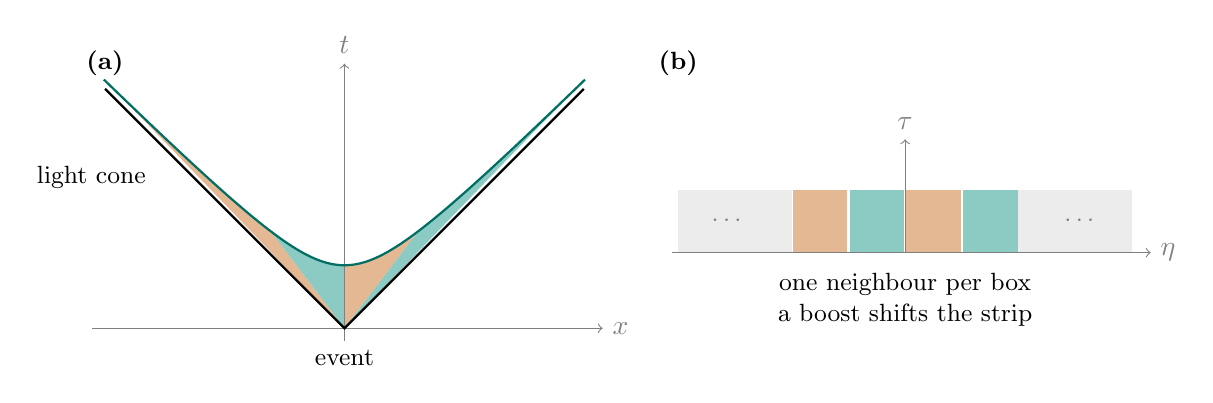
\begin{tikzpicture}[scale=0.8]
  \begin{scope}
  \foreach \a/\b/\c in {-2/-1/bandB, -1/0/bandA, 0/1/bandB, 1/2/bandA}{
    \fill[\c!45] (0,0) -- plot[domain=\a:\b,samples=40,variable=\e] ({sinh(\e)},{cosh(\e)}) -- cycle;
  }
  \draw[->,gray] (-4,0) -- (4.1,0) node[right] {$x$};
  \draw[->,gray] (0,-0.2) -- (0,4.2) node[above] {$t$};
  \draw[thick] (-3.8,3.8) -- (0,0) -- (3.8,3.8);
  \draw[thick,bandA!80!black] plot[domain=-2.05:2.05,samples=80,variable=\e] ({sinh(\e)},{cosh(\e)});
  \node[font=\small,anchor=east] at (-3.0,2.4) {light cone};
  \node[font=\small,anchor=north] at (0,-0.2) {event};
  \node[font=\small\bfseries] at (-3.8,4.2) {(a)};
  \end{scope}
  \begin{scope}[xshift=8.9cm,yshift=1.2cm]
  \foreach \a/\c in {-2/bandB,-1/bandA,0/bandB,1/bandA}{
    \fill[\c!45] (\a*0.9,0) rectangle ({(\a+1)*0.9},1);
    \draw[white,thick] (\a*0.9,0) -- (\a*0.9,1);
  }
  \fill[gray!15] (-3.6,0) rectangle (-1.8,1);
  \fill[gray!15] (1.8,0) rectangle (3.6,1);
  \node[gray,font=\small] at (-2.8,0.5) {$\cdots$};
  \node[gray,font=\small] at (2.8,0.5) {$\cdots$};
  \draw[->,gray] (-3.7,0) -- (3.9,0) node[right] {$\eta$};
  \draw[->,gray] (0,0) -- (0,1.8) node[above] {$\tau$};
  \node[font=\small,align=center] at (0,-0.75) {one neighbour per box\\a boost shifts the strip};
  \node[font=\small\bfseries] at (-3.6,3.0) {(b)};
  \end{scope}
\end{tikzpicture}
\caption{(a) Where the neighbours of an event live: near the light cone, coloured by rapidity band. (b) The same region in coordinates $(\eta,\tau)$: an infinite strip of equivalent boxes, each containing one neighbour on average. A boost slides the strip sideways like a conveyor belt.}
\label{fig:belt}
\end{figure}

\paragraph{The dilemma.} \lit{} This is the elementary core of a theorem of Bombelli, Henson and Sorkin~\cite{BHS06}: no discrete structure can give each event finitely many neighbours without singling out a frame. The reason is that a normalisable distribution cannot be uniform in rapidity, because rapidity, unlike angle, has no end. Lorentz-invariant discreteness is therefore non-local~\cite{Sorkin07}. Attempts to escape by making the points ``quantum blurry'' run into the same obstruction: a single neighbour in superposition over all rapidity bands, with equal weights as boost invariance demands, cannot be normalised.

\section{The cosmological cutoff}
\subsection{What rapidity is}
\est{} Rapidity $\eta$ is the natural measure of a boost. Velocity is $v=\tanh\eta$ and the Lorentz factor is $\gamma=\cosh\eta$. Unlike velocities, rapidities simply \emph{add} under successive boosts along a line. A boost by $\eta$ stretches one light-cone direction by $e^{\eta}$ and squeezes the other by $e^{-\eta}$. Some reference points:
\begin{center}\small
\begin{tabular}{@{}lll@{}}
\toprule
 & $\gamma$ & $\eta\approx\ln 2\gamma$ \\
\midrule
Earth relative to the CMB frame (370 km/s) & $1+10^{-6}$ & $0.0012$\\
LHC proton (6.8 TeV) & $7\times10^{3}$ & $9.6$\\
GZK threshold proton ($5\times10^{19}$ eV) & $5\times10^{10}$ & $25$\\
Highest-energy cosmic ray ($3.2\times10^{20}$ eV, if a proton) & $3.4\times10^{11}$ & $27$\\
\textbf{Cutoff $\eta_{\max}$ (this note)} & $\sim10^{61}$ & $\mathbf{142}$\\
\bottomrule
\end{tabular}
\end{center}
The GZK suppression of cosmic rays~\cite{CG99} is a genuine kinematic test at $\eta\approx25$. It requires that a CMB photon, seen from the rest frame of a $\gamma\sim10^{11}$ proton, has the boosted energy predicted by Lorentz transformations, and the observed suppression is consistent with that.

\subsection{A finite universe caps the rapidity}
\ours{} A neighbour at proper time $\tau$ and rapidity $\eta$ lies at spatial distance $r=\tau\sinh\eta\approx(\tau/2)\,e^{\eta}$ from the event. In a universe of size $L$ this cannot exceed $L$, so
\begin{equation}
\eta_{\max}\simeq\ln\frac{2L}{\tau}\approx\ln\frac{2L}{\lP}\approx142,
\end{equation}
using $L\approx4.4\times10^{26}$\,m (radius of the observable universe) and $\tau\sim\lP=1.6\times10^{-35}$\,m. Physically, $\eta_{\max}$ is the most extreme boost under which a Planck-sized neighbourhood still fits inside the universe: $e^{142}\approx10^{61.7}\approx2L/\lP$. Because the dependence on the inputs is logarithmic, the number is robust. Changing $L$ or the discreteness scale by a factor $10^{10}$ shifts it by only $\pm23$.

By Eq.~\eqref{eq:onepereta}, an event in $1+1$ dimensions has about $2\eta_{\max}\approx280$ future neighbours. That is finite and small. In $3+1$ dimensions the space of boost directions is a hyperboloid whose area grows like $\sinh^2\eta$. With $d^4x=\tau^3\sinh^2\!\eta\,d\tau\,d\eta\,d\Omega$ and causal-interval volume $\pi\tau^4/24$,
\begin{equation}
N^{(3+1)}_{\rm links}\approx2\pi\rho L^2\int_0^\infty\tau\,e^{-\rho\pi\tau^4/24}d\tau=\frac{\pi\sqrt{24}}{2}\Big(\frac{L}{\lP}\Big)^2\approx10^{124}.
\end{equation}

\subsection{What the cutoff buys}
\begin{itemize}[leftmargin=*,itemsep=2pt]
\item \textbf{A finite neighbour count, set by cosmology.} It is small in $1+1$ dimensions and huge in $3+1$.
\item \textbf{A preferred frame of the right kind.} The only frame singled out is that of the universe as a whole, cf.\ the compact-space twin paradox~\cite{BarrowLevin01}. That is a frame of the \emph{state}, compatible with R3. In relational terms it is the frame of the universe's own longest causal chain.
\item \textbf{Consistency with experiment.} Local Lorentz invariance holds for $\eta\ll142$. Tests reach $\eta\approx25$--$27$.
\item \textbf{Causality intact.} All neighbours are inside the light cone. The non-locality is ``light-cone shaped'': the emission and absorption of a photon from a distant galaxy are almost neighbours.
\end{itemize}

\section{Relations only: a background-free toy model}
To comply with R2 we analyse a finite $1+1$ ``universe'', a causal diamond, using only its order relation. As in causal set theory, we generate test configurations by Poisson sprinkling, a stand-in for unknown dynamics, and then discard all coordinates. In light-cone coordinates a sprinkled diamond is equivalent to a random permutation, which makes two exact statements available.

\paragraph{Proper time by counting.} \lit{} The proper time between the tips of the diamond is estimated by the length $\mathcal L$ of the longest causal chain~\cite{BrightwellGregory91}. In $1+1$ dimensions this is the longest increasing subsequence of a random permutation (Ulam's problem), for which $\langle\mathcal L\rangle\simeq2\sqrt n-1.77\,n^{1/6}$ with Tracy--Widom fluctuations $\delta\mathcal L\simeq0.90\,n^{1/6}$~\cite{BDJ99}. With $n=\rho\tau^2/2$ this gives
\begin{equation}
\frac{\delta\tau}{\tau}\simeq0.45\,n^{-1/3}.
\end{equation}
\ours{} (interpretation) This is the background-free version of our earlier ``quantum blur'' intuition: geometry measured by counting is \emph{intrinsically fuzzy}. The fuzziness is statistical, not yet quantum, and it is a relation between events, not a smearing in some background space.

\paragraph{Neighbours by counting.} \est{} The links of an event are the minimal elements of its future. Ordered along one light-cone direction, they are the running minima (``records'') along the other. For $m$ events in the future the expected number of records is the harmonic number $H_m=1+\tfrac12+\dots+\tfrac1m\simeq\ln m+0.577$. For an event at the centre of a diamond of $n$ events, $m\approx n/4$ and $\langle N_{\rm links}\rangle\simeq\ln n-0.81$. Since $\ln n\simeq2\ln(L/\lP)$, this is the $2\eta_{\max}$ of Sec.~3, now derived without any background.

\begin{table}[t]
\centering\small
\begin{tabular}{@{}rccccc@{}}
\toprule
$n$ & $\langle\mathcal L\rangle$ & $2\sqrt n$ & $\delta\mathcal L/n^{1/6}$ & $\langle N_{\rm links}\rangle$ & $\langle H_m\rangle$\\
\midrule
$10^2$ & 16.7 & 20.0 & 0.75 & 3.78 & 3.80\\
$10^3$ & 58.4 & 63.2 & 0.92 & 6.09 & 6.10\\
$10^4$ & 192.1 & 200.0 & 0.89 & 8.43 & 8.40\\
$10^5$ & 620.6 & 632.5 & 0.92 & 10.76 & 10.70\\
$10^6$ & --- & --- & --- & 13.04 & 13.01\\
\bottomrule
\end{tabular}
\caption{Numerics for sprinkled causal diamonds (\texttt{sims/causal\_diamond.py}; 100--2000 samples per row). The longest chain approaches $2\sqrt n$ with fluctuations $\approx0.9\,n^{1/6}$ (Tracy--Widom value $0.90$). The neighbour count of the central event matches the harmonic number, i.e.\ grows like $\ln n$.}
\label{tab:diamond}
\end{table}

\section{Growth: a universe that creates its events}
\lit{} If the number of events measures spacetime volume (``Number $=$ Volume''~\cite{Surya19}), an expanding universe must keep producing new events. In causal set theory this is literal: in sequential growth dynamics~\cite{RideoutSorkin00}, the passage of time \emph{is} the birth of new elements. In our picture the cutoff then grows with cosmic time,
\begin{equation}
\eta_{\max}(t)\simeq\ln\frac{2L(t)}{\lP},
\end{equation}
so the range over which Lorentz invariance holds widens as the universe grows, logarithmically and imperceptibly. Sorkin's heuristic that the cosmological constant fluctuates as $\Lambda\sim1/\sqrt N$~\cite{ADGS04} uses the same counting. Whether random creation of events produces exactly such fluctuations is open. To respect R2, creation rates must be defined by counting events in causal intervals, not by velocities of a flowing medium. An earlier ``river'' formulation was dropped for that reason (App.~\ref{app:dropped}).

\section{Discussion}
\paragraph{Where this sits.} The construction lies inside causal set theory: links, infinite valency, the Bombelli--Henson--Sorkin dilemma, Number $=$ Volume and growth are all theirs. Our only additions are (i) treating the finite size of the universe as the physical regulator of the non-locality, (ii) accepting the resulting cosmological frame as an explanation rather than a defect, and (iii) a pedagogical, fully elementary route to these statements. A brief search did not find (i) stated in this form, but it may exist.

\paragraph{Limitations.}
\begin{enumerate}[leftmargin=*,itemsep=1pt]
\item \emph{$3+1$ is not tamed.} $10^{124}$ neighbours per event is finite but hardly local. The $1+1$ result (about 280) is misleadingly mild.
\item \emph{No prediction yet.} The cutoff is unreachable by construction. Effects leaking down to observable rapidities would need dynamics we do not have. A naive guess $e^{-(\eta_{\max}-\eta)}$ gives about $10^{-50}$ at $\eta=27$.
\item \emph{No dynamics.} Nothing here yields Einstein's equations. Sprinkling stands in for unknown dynamics, and most random orders do not look like spacetime at all (the Kleitman--Rothschild problem~\cite{Surya19}).
\item \emph{The fuzziness is classical.} The $n^{1/6}$ fluctuations are statistical. A quantum version is not attempted.
\item \emph{``Size of the universe'' is ambiguous.} The Hubble radius, the particle horizon and the event horizon differ by $O(1)$ factors. Thanks to the logarithm this changes $\eta_{\max}$ by $O(1)$, but it must be defined relationally.
\end{enumerate}

\paragraph{Next steps.} (1) Define $L$, and hence $\eta_{\max}$, relationally in a growing causal set. (2) Ask whether a finite valency changes the behaviour of the causal-set wave operator~\cite{Sorkin07} in a way that could be observed. (3) Test whether random growth reproduces $\Lambda\sim1/\sqrt N$. (4) Repeat the toy model in $2+1$ and $3+1$ dimensions.

\appendix
\section{Paths explored and dropped}\label{app:dropped}
\begin{itemize}[leftmargin=*,itemsep=1pt]
\item \textbf{A regular crystal of events.} Polygonal light cones and a lattice rest frame (Sec.~2.1).
\item \textbf{Quantum blur of positions.} Blur in \emph{what}? It presupposes a background. It also cures the zero-measure problem but not the divergence, and an equal superposition over rapidity cannot be normalised.
\item \textbf{A quantum chain as the source of blur.} Positional zero-point fluctuations grow as $\ln N$ in one dimension. The model is background-dependent, and its claimed analogy with atomic linewidths was overstated.
\item \textbf{Exactly-one-tick neighbours on lattices with discrete boost symmetry} (Schild~\cite{Schild48}). These also give infinitely many neighbours. This confirms the dilemma but adds nothing beyond it.
\item \textbf{Expansion as a source and gravity as a sink of points} (river model~\cite{HamiltonLisle08}). It needs a preferred family of observers, i.e.\ an aether, which R2 forbids.
\item \textbf{A link to Bell non-locality.} Links join only timelike-separated events, while Bell correlations are spacelike. Wrong kind of non-locality.
\item \textbf{$(L/\lP)^2\sim10^{122}$ and the cosmological constant.} Numerology: every combination of $L$ and $\lP$ is a power of $10^{61}$.
\end{itemize}

\begin{thebibliography}{99}\small
\bibitem{JacobsonMattingly01} T.~Jacobson, D.~Mattingly, ``Gravity with a dynamical preferred frame'', Phys.\ Rev.\ D 64, 024028 (2001), gr-qc/0007031.
\bibitem{Burago} D.~Burago, ``Periodic metrics''; statement in arXiv:1104.4460.
\bibitem{Weyl} H.~Weyl, \emph{Philosophy of Mathematics and Natural Science} (1949).
\bibitem{VahidiAslWierman} M.~Q.~Vahidi-Asl, J.~C.~Wierman, in \emph{Random Graphs 87} (1990) and \emph{Random Graphs 89} (1992).
\bibitem{BLMS87} L.~Bombelli, J.~Lee, D.~Meyer, R.~D.~Sorkin, ``Space-time as a causal set'', Phys.\ Rev.\ Lett.\ 59, 521 (1987).
\bibitem{Surya19} S.~Surya, ``The causal set approach to quantum gravity'', Living Rev.\ Rel.\ (2019), arXiv:1903.11544.
\bibitem{BHS06} L.~Bombelli, J.~Henson, R.~D.~Sorkin, ``Discreteness without symmetry breaking: a theorem'', gr-qc/0605006.
\bibitem{Sorkin07} R.~D.~Sorkin, ``Does locality fail at intermediate length-scales?'', gr-qc/0703099.
\bibitem{CG99} S.~Coleman, S.~L.~Glashow, ``High-energy tests of Lorentz invariance'', Phys.\ Rev.\ D 59, 116008 (1999), hep-ph/9812418.
\bibitem{BarrowLevin01} J.~D.~Barrow, J.~Levin, ``The twin paradox in compact spaces'', Phys.\ Rev.\ A 63, 044104 (2001).
\bibitem{BrightwellGregory91} G.~Brightwell, R.~Gregory, ``Structure of random discrete spacetime'', Phys.\ Rev.\ Lett.\ 66, 260 (1991).
\bibitem{BDJ99} J.~Baik, P.~Deift, K.~Johansson, ``On the distribution of the length of the longest increasing subsequence of random permutations'', J.\ Amer.\ Math.\ Soc.\ 12, 1119 (1999).
\bibitem{RideoutSorkin00} D.~P.~Rideout, R.~D.~Sorkin, ``A classical sequential growth dynamics for causal sets'', Phys.\ Rev.\ D 61, 024002 (2000).
\bibitem{ADGS04} M.~Ahmed, S.~Dodelson, P.~Greene, R.~D.~Sorkin, ``Everpresent $\Lambda$'', Phys.\ Rev.\ D 69, 103523 (2004).
\bibitem{Schild48} A.~Schild, ``Discrete space-time and integral Lorentz transformations'', Phys.\ Rev.\ 73, 414 (1948).
\bibitem{HamiltonLisle08} A.~J.~S.~Hamilton, J.~P.~Lisle, ``The river model of black holes'', Am.\ J.\ Phys.\ 76, 519 (2008).
\end{thebibliography}
\end{document}
